\label{sec:vbf-likelihood}

\subsubsection{Yield and likelihood}
The negative log-likelihood is constructed as shown in Equation~\ref{likelihood}, 
where $Y_{ijk}$ denotes the yield of $k^{th}$ bin of $j^{th}$ region of $i^{th}$ channel. 
Nuisance parameters, which have external constraints $f(\alpha_l)$, are penalized in the negative log-likelihood. 

Both \twocentral{} and  \fourcentral{} channel consists of four signal regions and yield in total eight \Mbb{} distributions.
The yield of a given region R is calculated with Equation~\ref{yield_float}. Note in the equation that a Gaussian constraint $\alpha_{sp}$  for spurious signal is included with width being the spurious signal size we measured in the spurious signal test.

Free parameters are the normalizations of the non-resonant background in each control and
signal region, denoted with $N_B$.
The signal normalizations $N_H$ are set to the Standard Model expectation from simulation,
while $\mu$ represents the observed signal strength.
The shapes of Higgs, Z and non-resonant background are $H$, $Z$ and $B$, respectively.

\begin{equation}
\label{likelihood}
-\log\mathcal{L}(\mu, \{\alpha_{l}\} )= -\log \prod_{i=1}^{\textnormal{Channels}} \prod_{j=1}^{\textnormal{Regions}} \prod_{k=1}^{\textnormal{Bins}} \frac{e^{-Y_{ijk}(\mu, \{\alpha_l\})} \times Y_{ijk}N_{ijk}^{Obs} }{N_{ijk}^{Obs}} - \log \prod_{l}^{\textnormal{Nuisance Pars}} f(\alpha_l)
\end{equation}

\begin{equation}
\label{yield_float}
\begin{split}
Y(R) &= (\mu + \alpha_{sp}(R))N_{H}H(R)+ N_{B}B(R)+ \mu_{z}(R)N_{Z}Z  \\
\end{split}
\end{equation}


Eq.\ref{yield_float} adopts the strategy floating the $Z$ contributions in all BDT regions. 


%In case we adopt the method only floating the $Z$ contributions in SR I and SR II of \twocentral, the rest of the regions will have yield as in Eq.\ref{yield_constrain} where $\mu_z(Norm)$ stands for the floating parameters for $Z$ normalization and $\alpha_z(R)$ stands for the BDT shape nuisance parameter with 50\% width. 

%\begin{equation}
%\label{yield_constrain}
%\begin{split}
%Y(R) &= (\mu + \alpha_{sp}(R))N_{H}H(R)+ N_{B}B(R)+ \mu_{z}(Norm)\alpha_z(R)N_{Z}Z  \\
%\end{split}
%\end{equation}



%The nuisance parameter $\alpha_{z}$ controls the overall normalization for the \zjets{} template 
%and is constrained with a Gaussian prior with width 0.06. The overall normalization is scaled
% to 0.81 and 0.75 for \twocentral and \fourcentral channels, respectively, determined as described in Section~\ref{sec:vbf-ztreat}..
%We also adopt independent NPs for each BDT region to account the data/MC shape difference of \zjets{}. 
%The chosen values are motivated by the validation study in data described in Appendix~\ref{sec:vbf-zjets}. 


\subsubsection{Fits on toy experiments}

To determine if the fit procedure yields bias, we build 2000 toy experiments from the background function determined in the background only fit and inject the \zjets{} component fixed at the Standard Model prediction. The Higgs signals of different strengths are injected at $\mu_{inj} = 0.5, 1.0, 2.0, 5.0$. The pulls of the toy experiment fits defined as $(\mu_{fit}-\mu_{inj})/ \sigma$ are shown in Figures \ref{fig:MCToy}. The distributions of pulls are fitted with Gaussian distribution to determine means and widths, which are consistent with 0 and 1, respectively, within statistical uncertainties. For $\mu_{inj}=1.0$ test, we fit back $\hat{\mu}=1.0\pm 1.9$. %treating all NPs except the analytical background parameterization and normalization as systeamtics. 
The expected signal significance in this case is 0.5. The dominant uncertainty is statistical which encompasses the normalization and parameterization of the non-resonant background. The Z signal strength is shown in Table \ref{tab:zstrength}. The effective combined Z signal strength is $1.0\pm 0.1$. %(If we adopt the strategy to only float the $Z$ contribution in SR I and SR II of \twocentral channel, we get $\hat{\mu}=1.00\pm 1.35$). 

\begin{figure}[htbp]
  \centering
 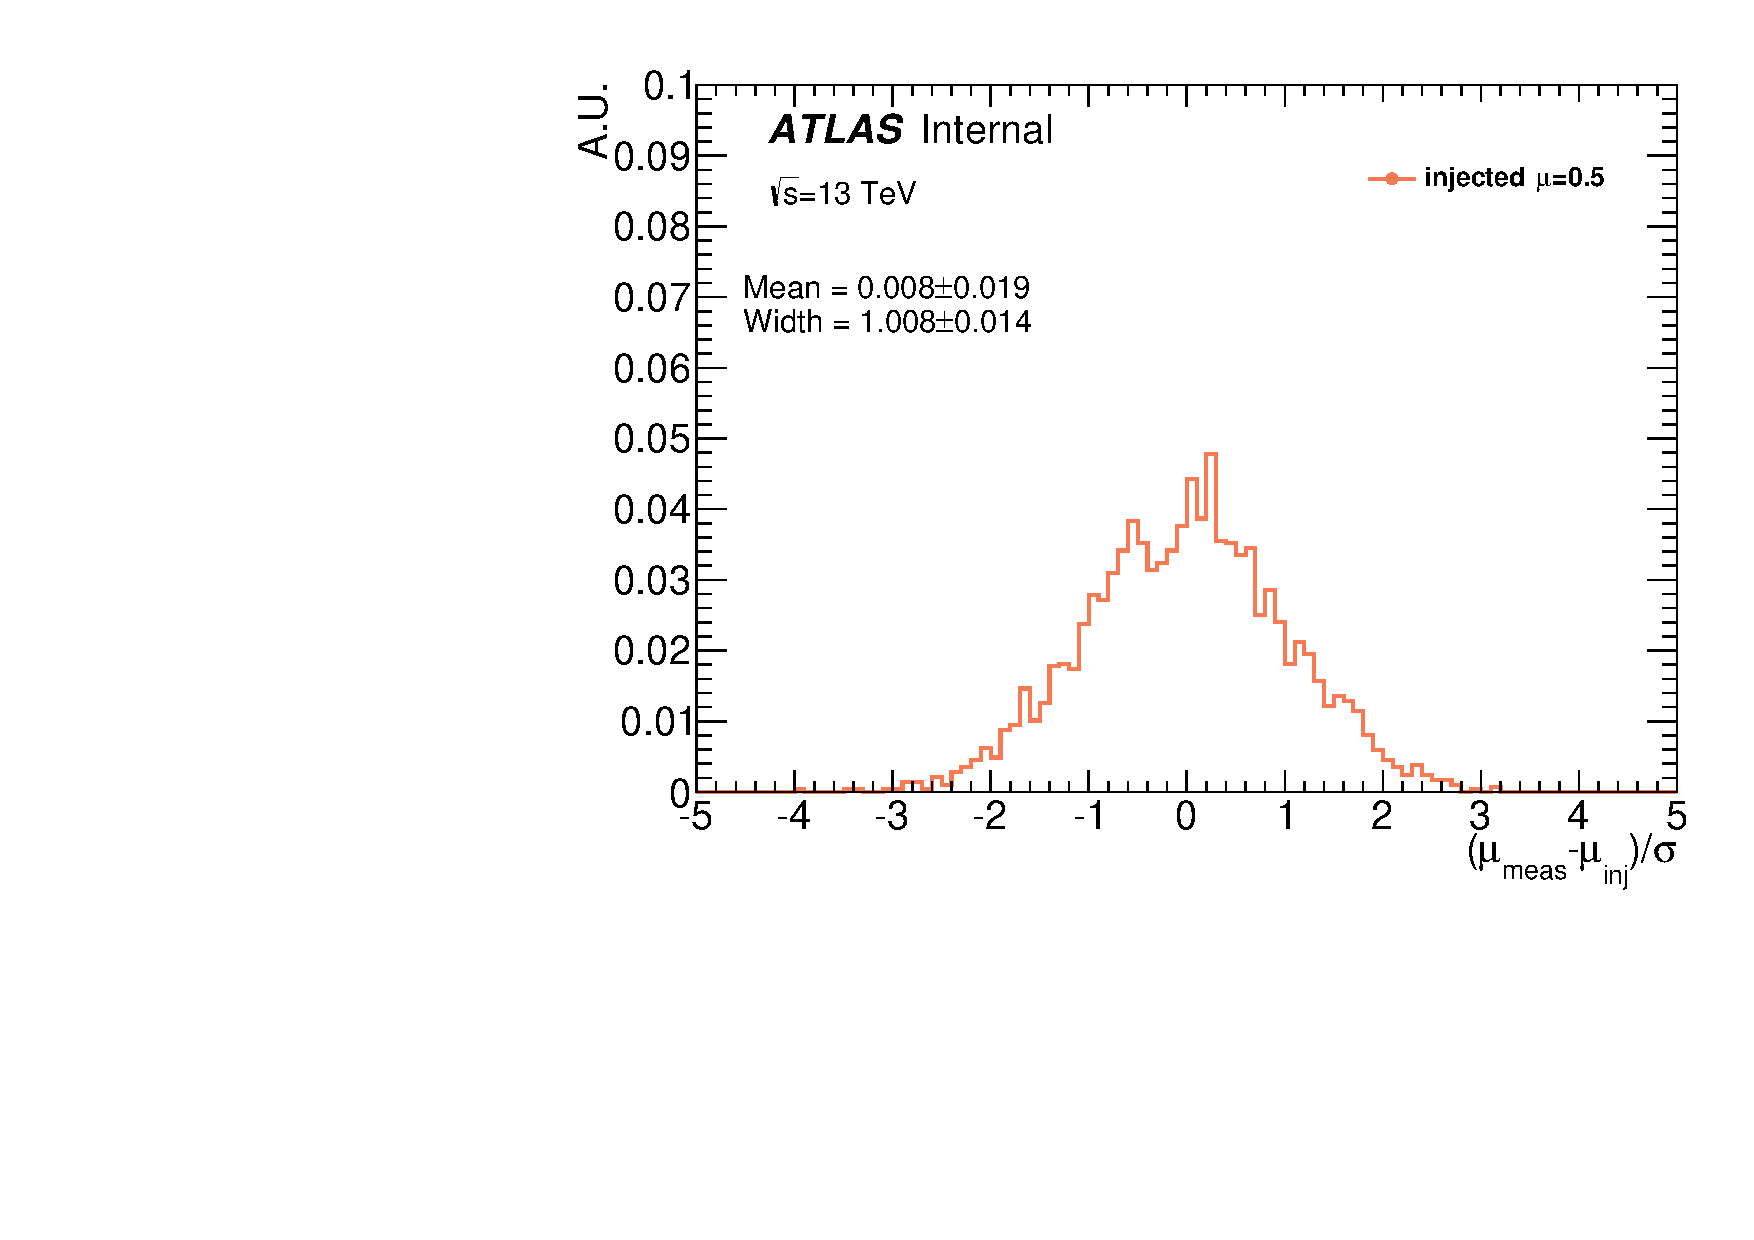
\includegraphics[width=0.45\textwidth]{figures/VBF/Mu05.pdf}
 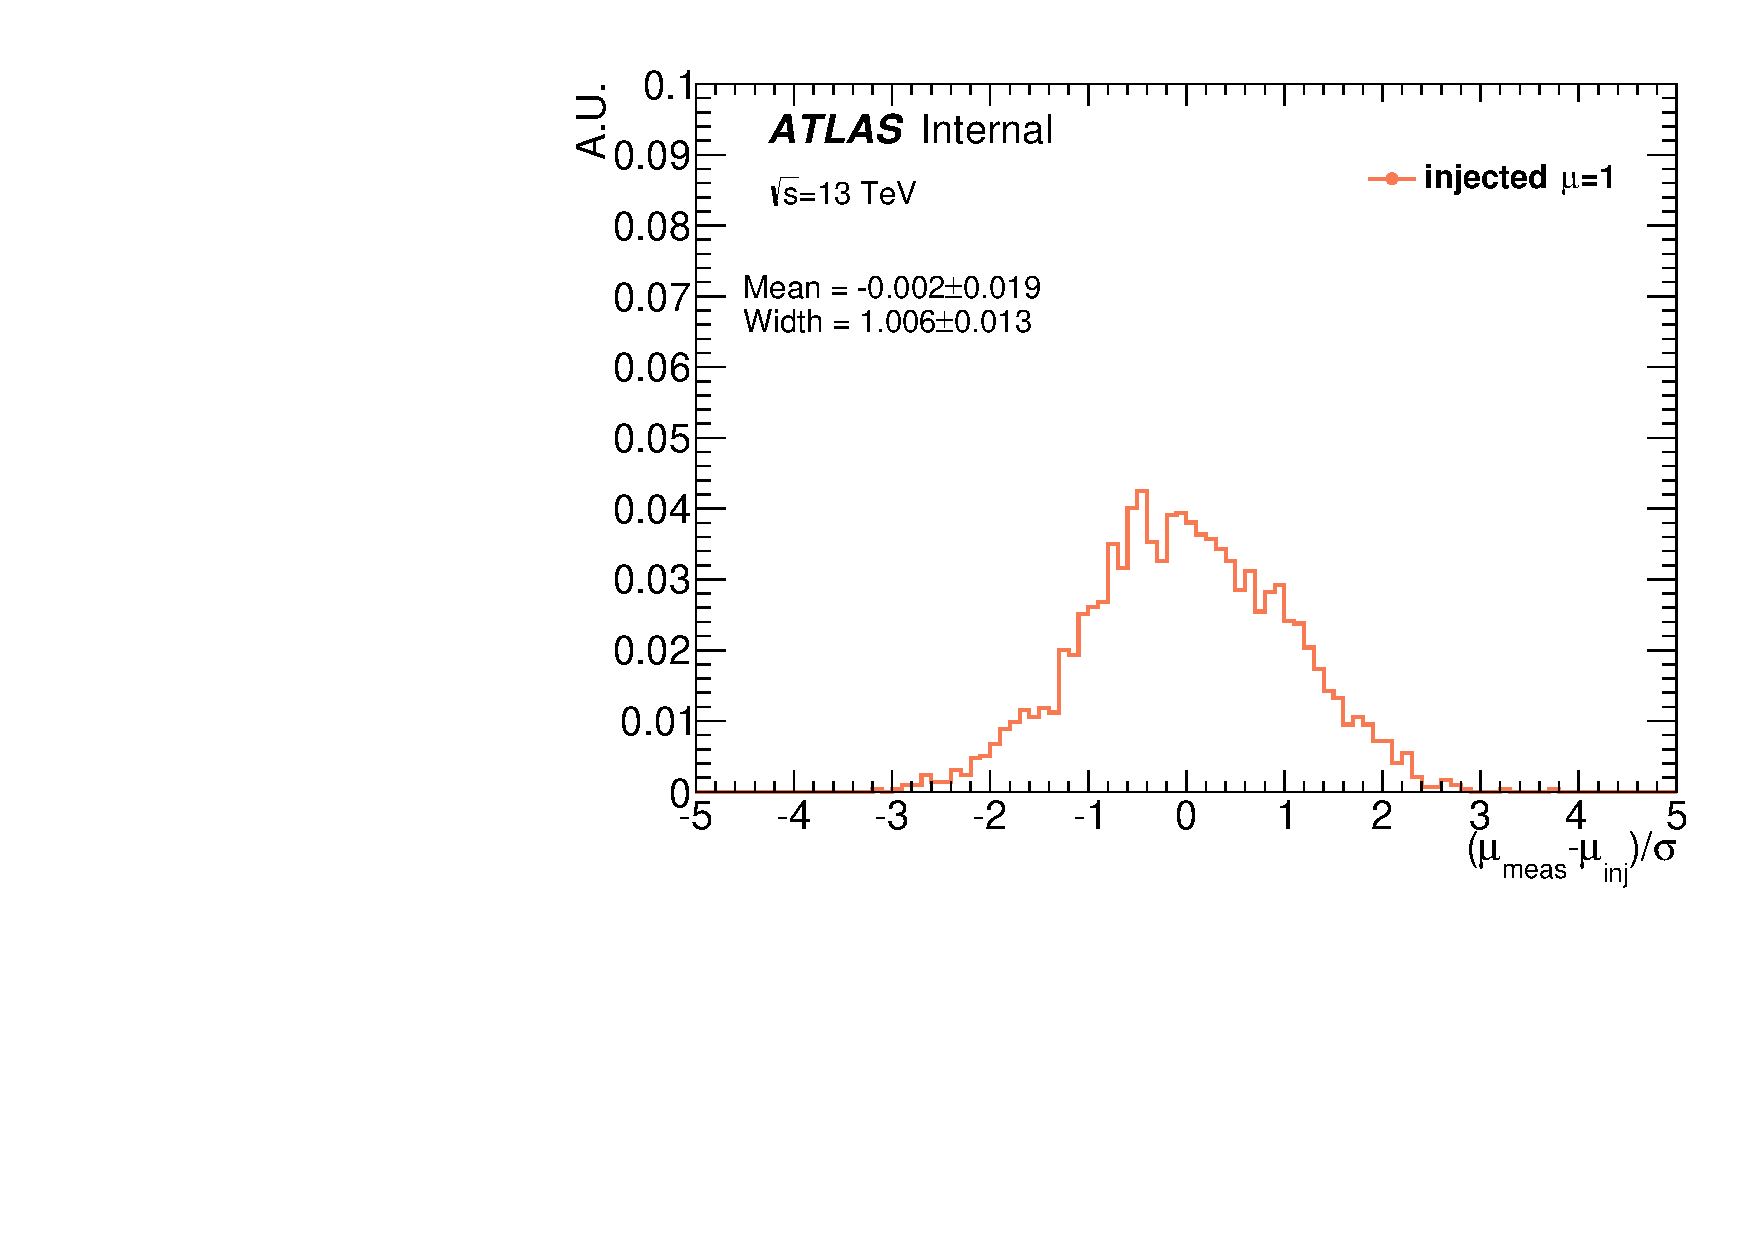
\includegraphics[width=0.45\textwidth]{figures/VBF/Mu1.pdf}\\
 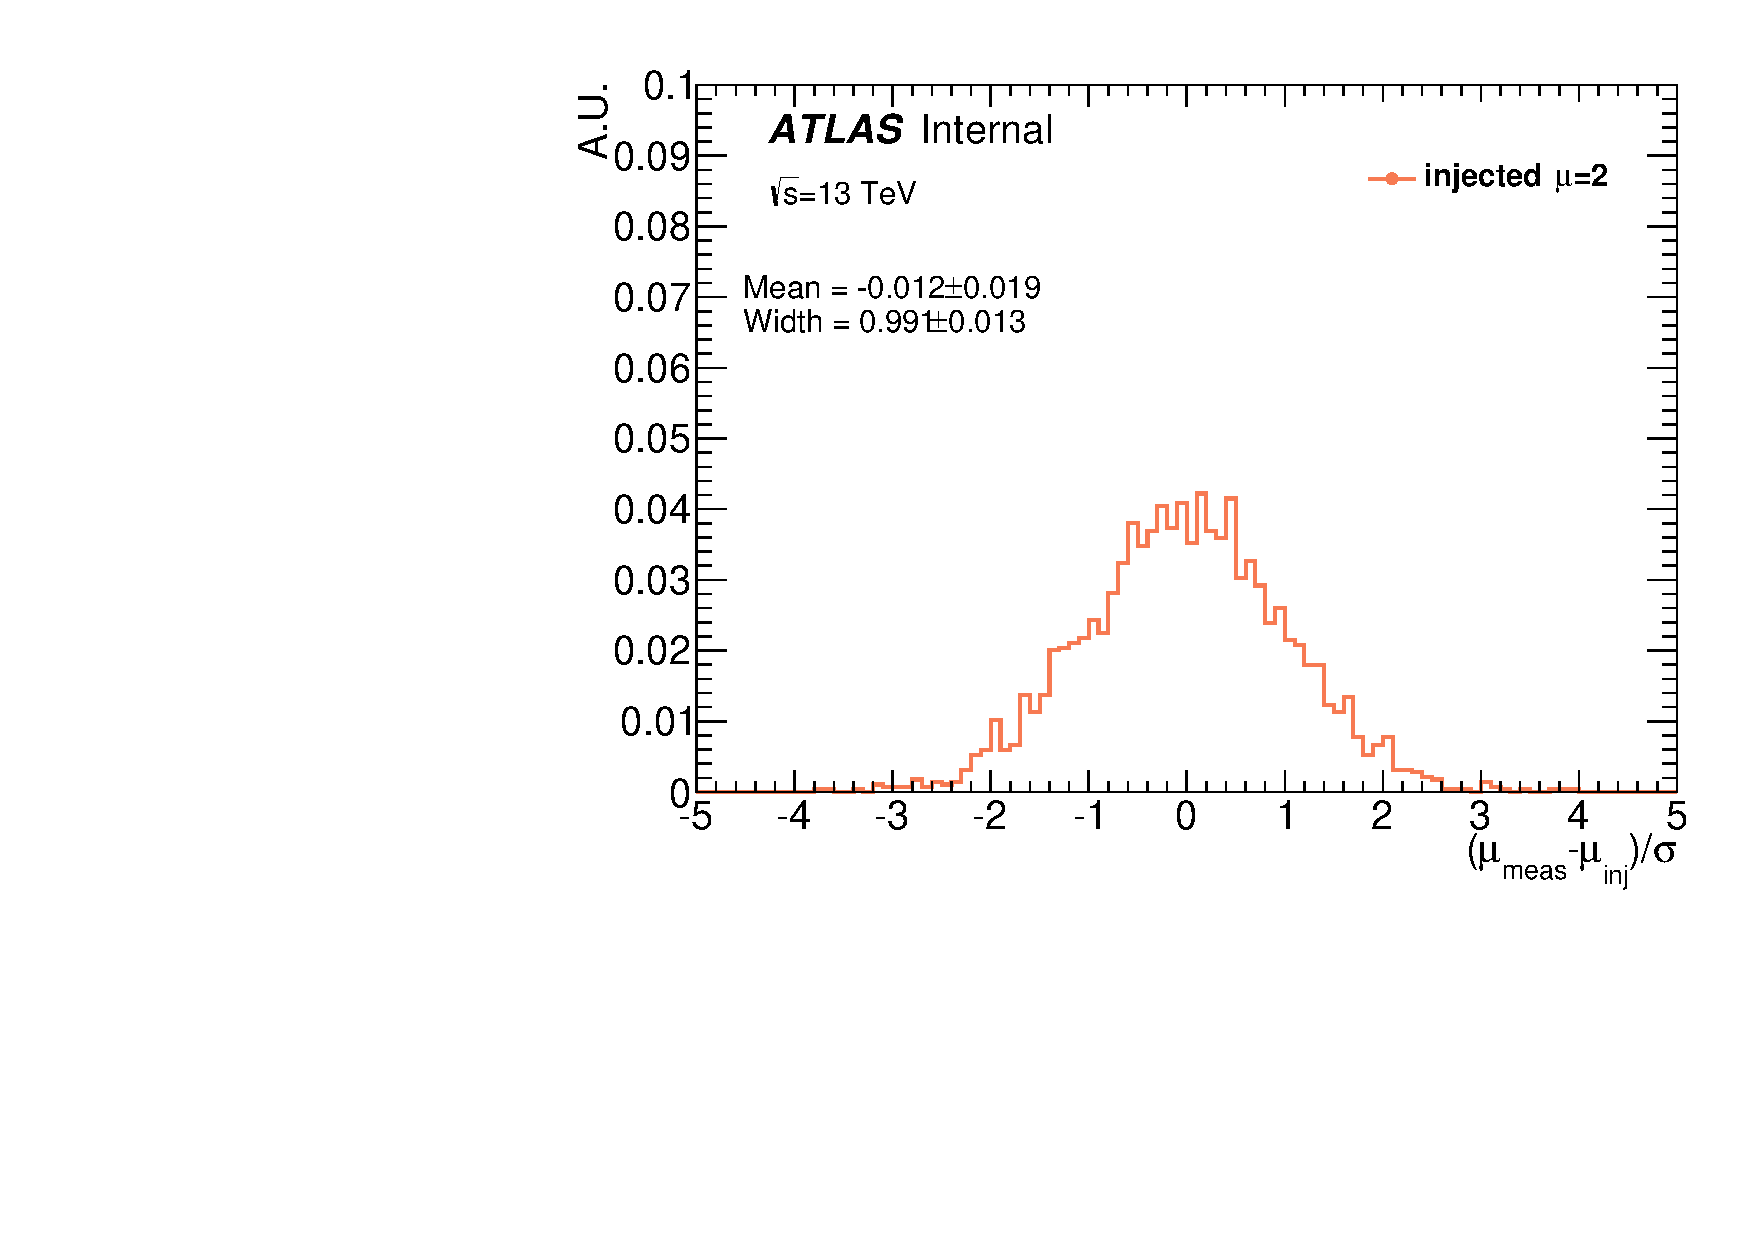
\includegraphics[width=0.45\textwidth]{figures/VBF/Mu2.pdf}
 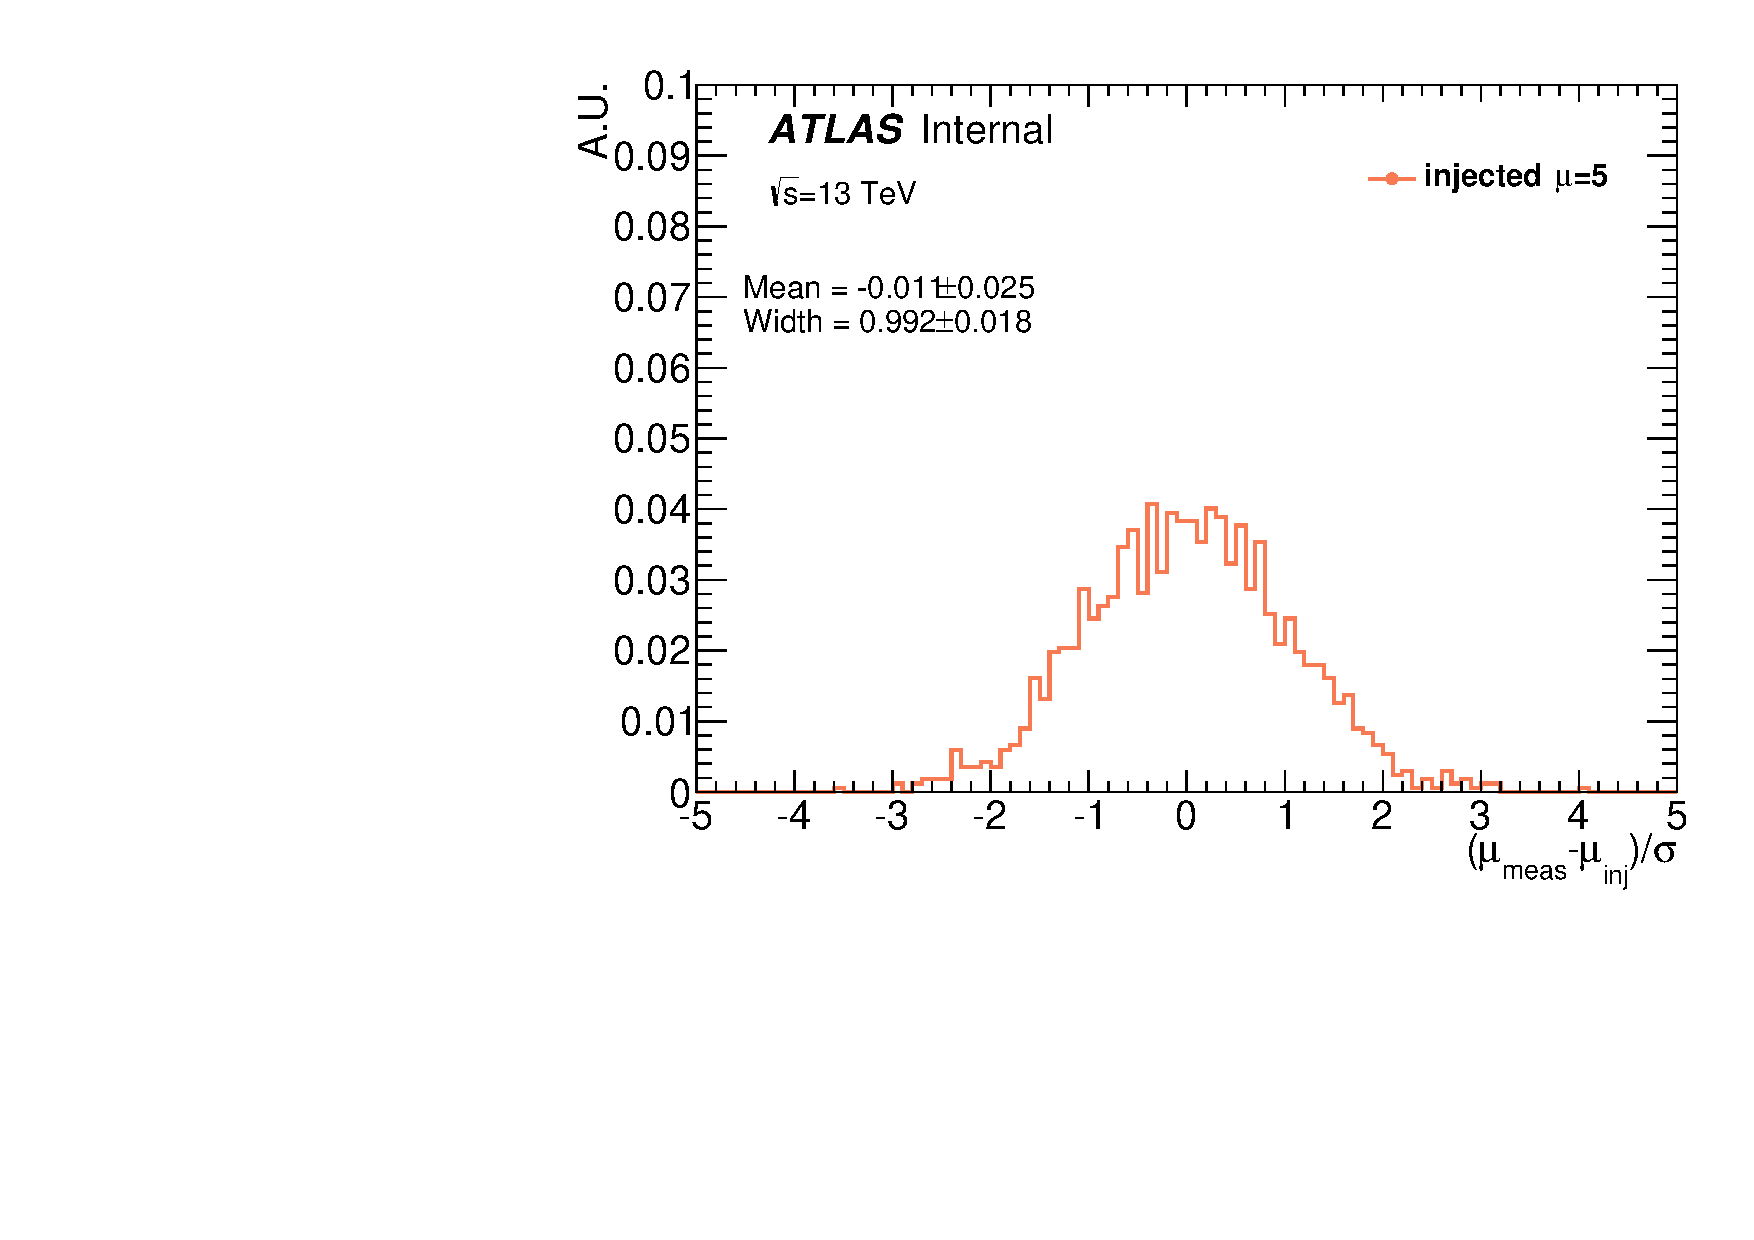
\includegraphics[width=0.45\textwidth]{figures/VBF/Mu5.pdf}\\
\caption{Pull distribution of toy experiment fits. We inject Higgs signal strength of 0.5 (top left), 1.0 (top right), 2.0 (bottom left) and 5.0 (bottom right) times the Standard Model prediction. The pulls are fitted with Gaussian to determine the means and widths which are unbiased. }
  \label{fig:MCToy}
\end{figure}

\begin{table}[htbp]
\centering
\caption{Floating Z normalization parameters in Asimov fit}
\label{tab:zstrength}
\begin{tabular}{|c|c|}
\hline
Region               & Asimov fit Z signal strength \\ \hline
SR I, \twocentral    & $ 1.00 \pm 0.7$              \\ \hline
SR II, \twocentral   & $ 1.00 \pm 0.5$             \\ \hline
SR I, \fourcentral   & $ 1.00 \pm 1.1$             \\ \hline
SR II, \fourcentral  & $ 1.00 \pm 0.6$             \\ \hline
SR III, \fourcentral & $ 1.00 \pm 0.3$             \\ \hline
SR IV, \fourcentral  & $ 1.00 \pm 0.2$             \\ \hline
\end{tabular}
\end{table}



%The uncertainties and pulls in the fit are shown in Figure~\ref{fig:pull_asimov} and the correlation matrix is shown in Figure~\ref{fig:corr_asimov}.
The fit correlation matrix is shown in Figure~\ref{fig:corr_asimov}. We observe, as expected, the Higgs signal is mildly anti-correlated with background normalization, Z strength and spurious signal size. The Z signal strength also shows as expected to be anti-correlated to background normalization given the degeneracy between the Z mass region and the low-mass sideband. The background parameters within a given channel are highly correlated as the variation of the contribution of one base function will need the variation of other bases to maintain the same background shape. 


%\begin{figure}[htbp]
%  \centering
% 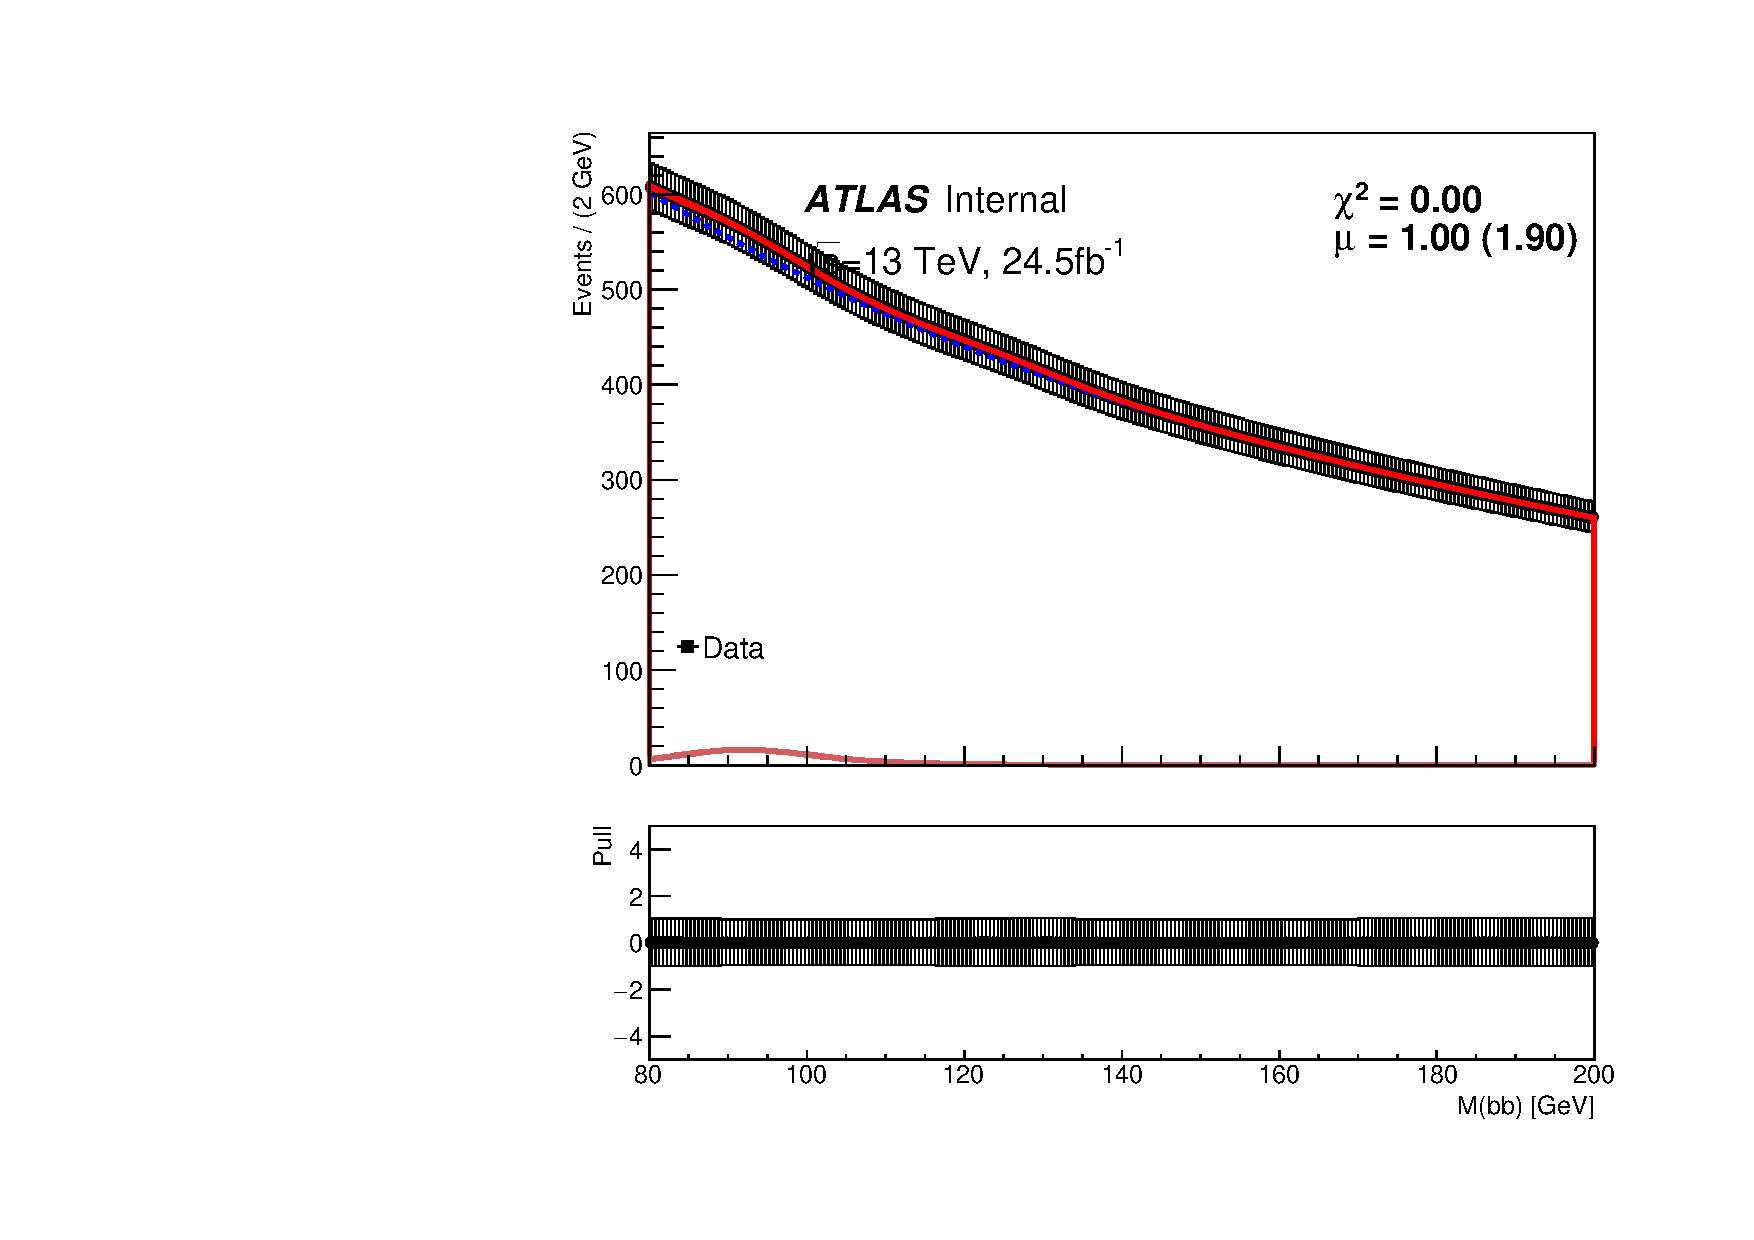
\includegraphics[width=0.48\textwidth]{figures/VBF/Asimov_testVBF_ICHEP_2cen_SRI.pdf}
% 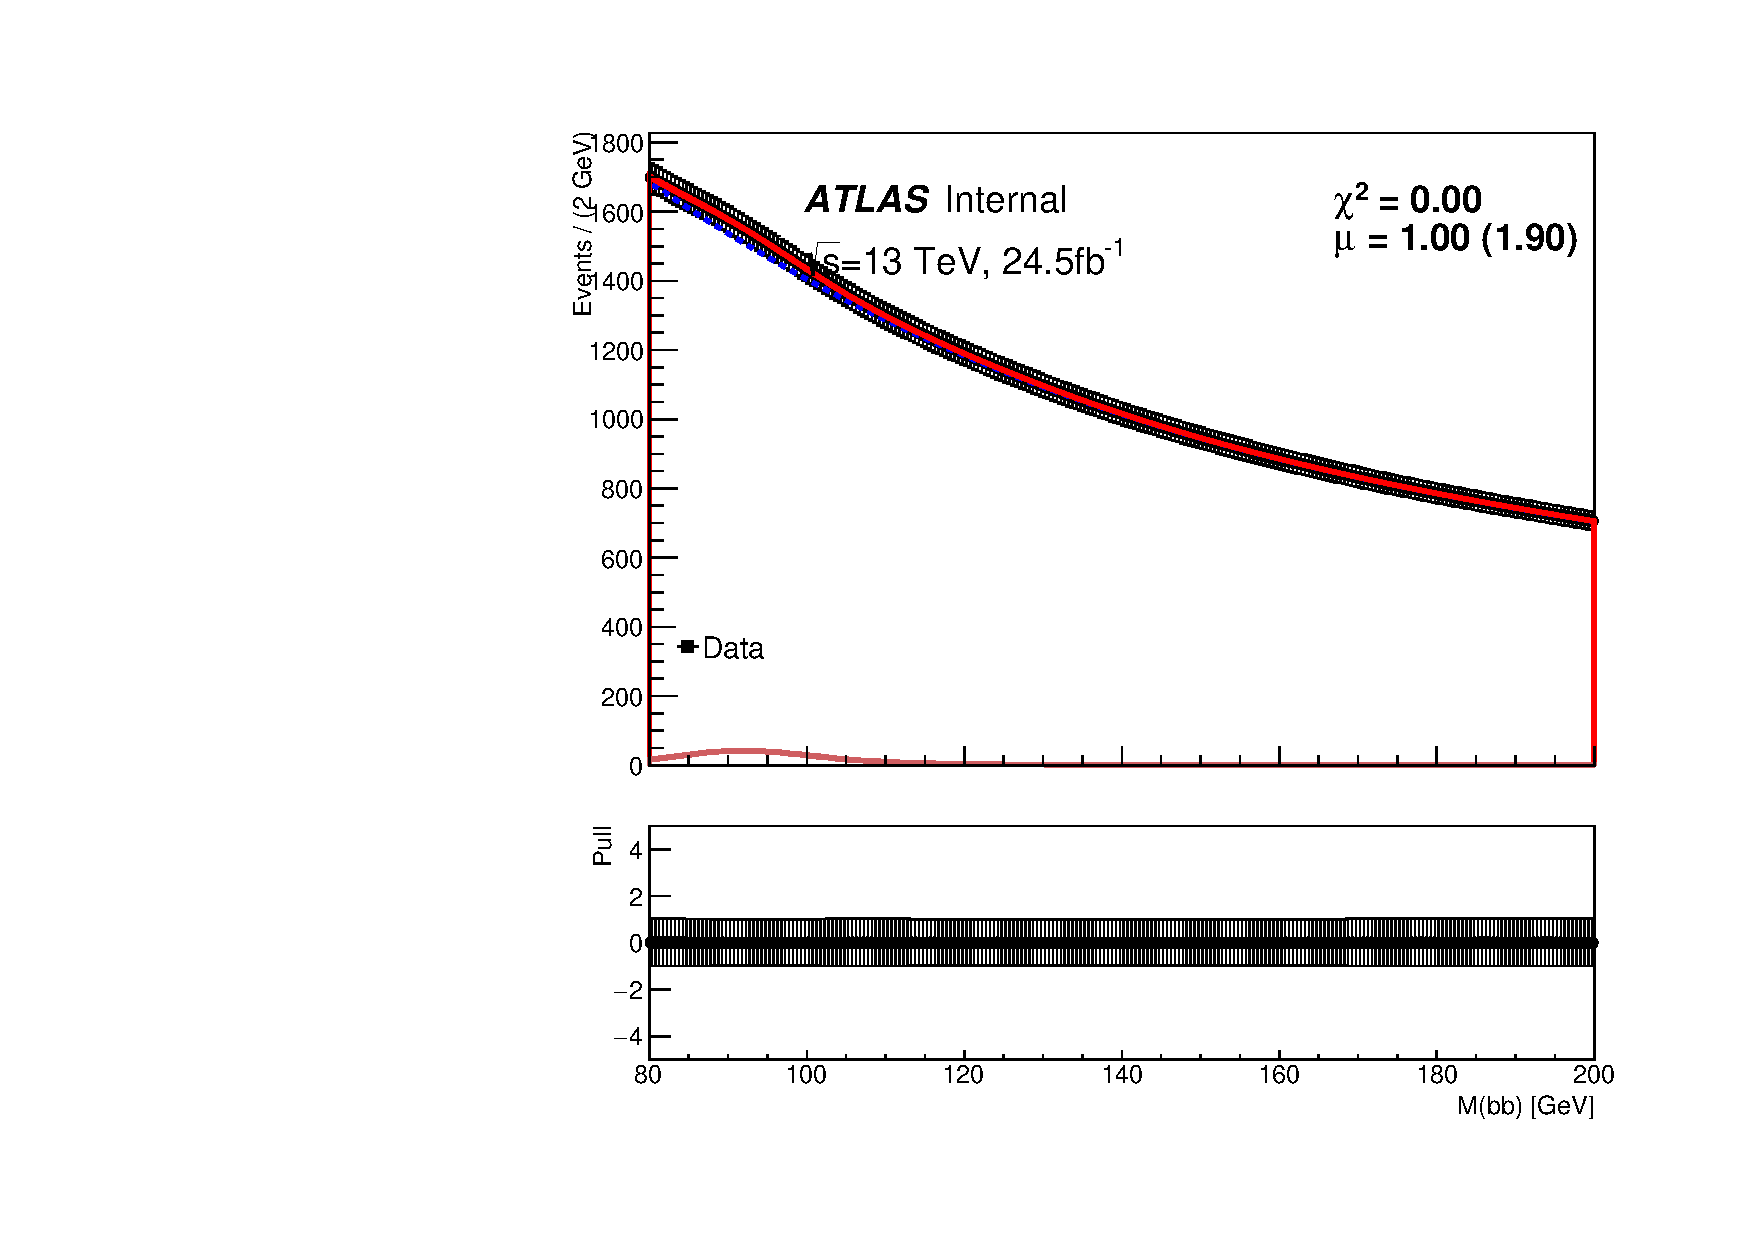
\includegraphics[width=0.48\textwidth]{figures/VBF/Asimov_testVBF_ICHEP_2cen_SRII.pdf}\\
%\caption{Asymptotic Asimov fits for SRI and SRII for the \twocentral channel.}
%  \label{fig:2cenAsimov}
%\end{figure}
%
%\begin{figure}[htbp]
%  \centering
% 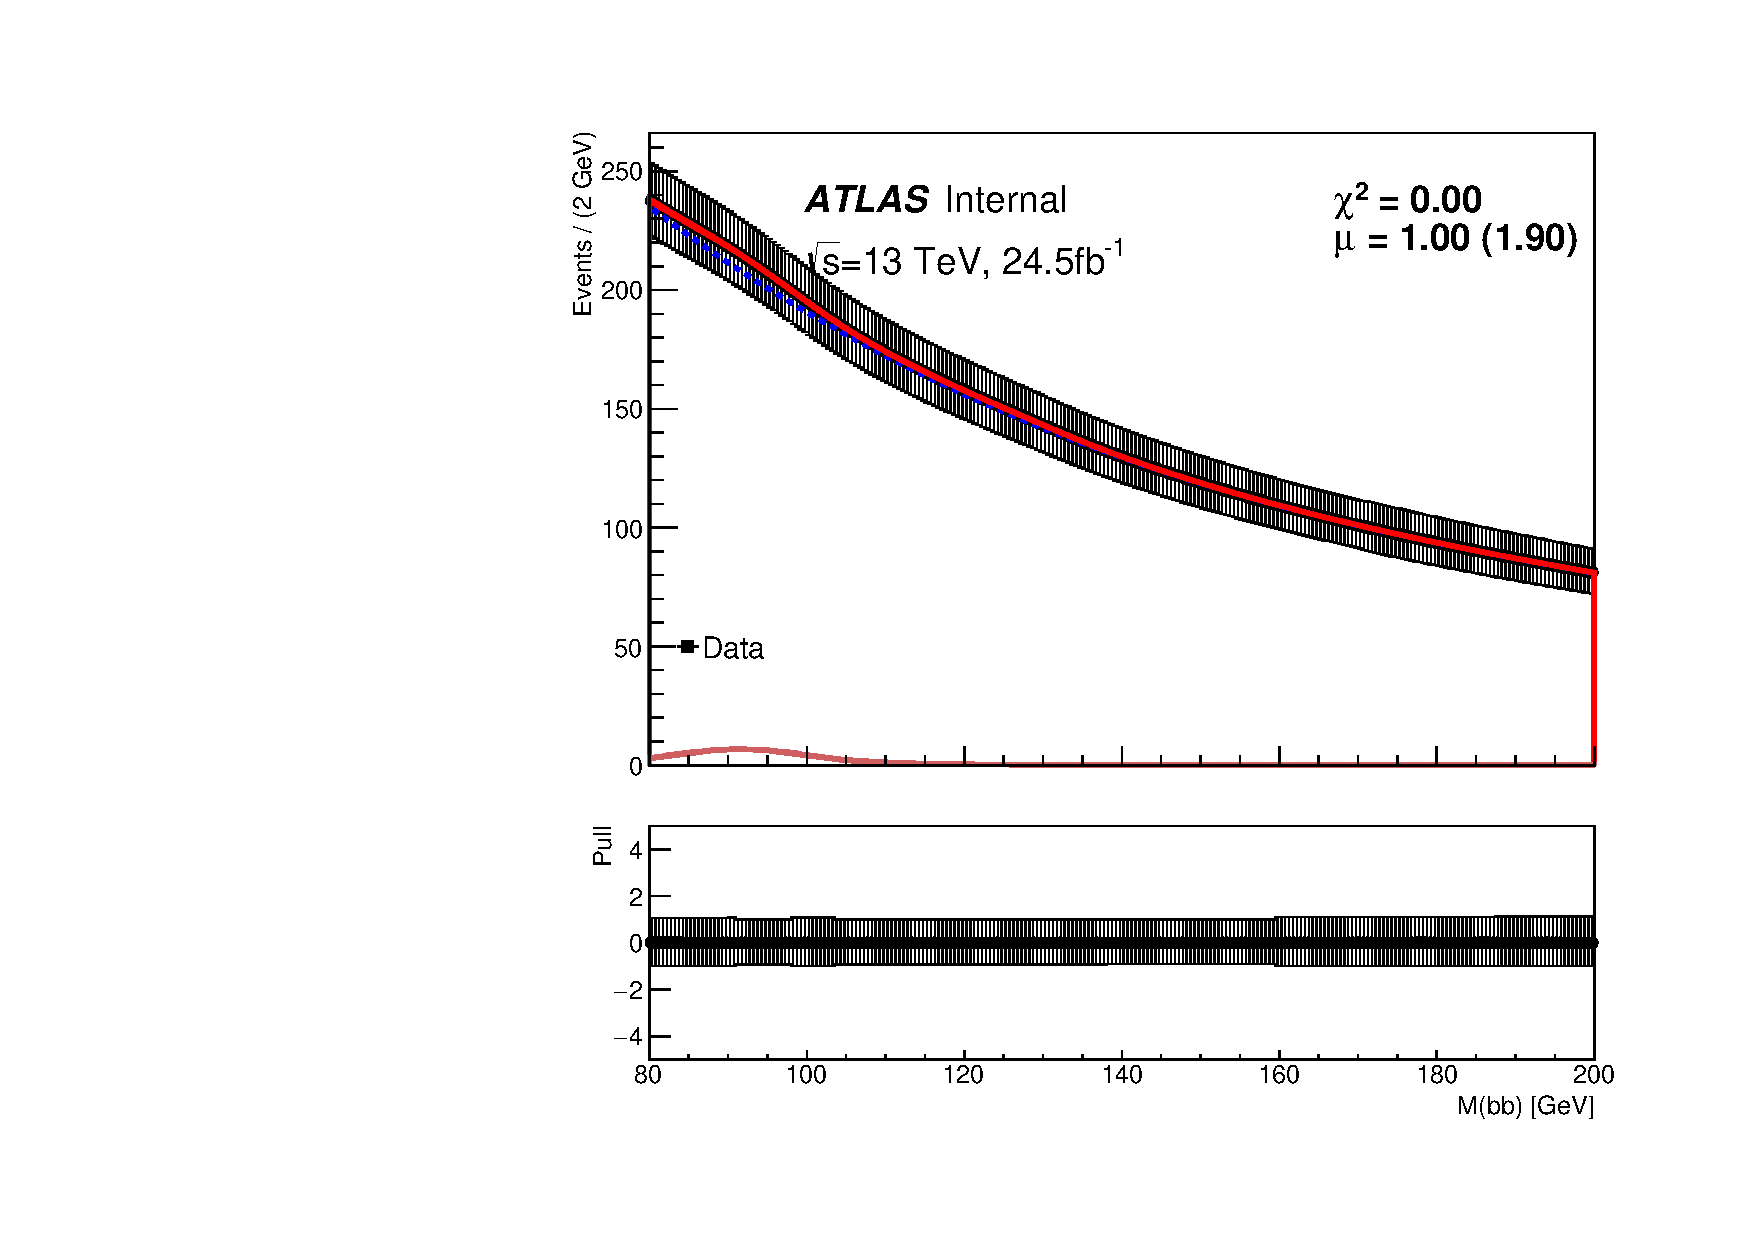
\includegraphics[width=0.48\textwidth]{figures/VBF/Asimov_testVBF_ICHEP_4cen_SRI.pdf}
% 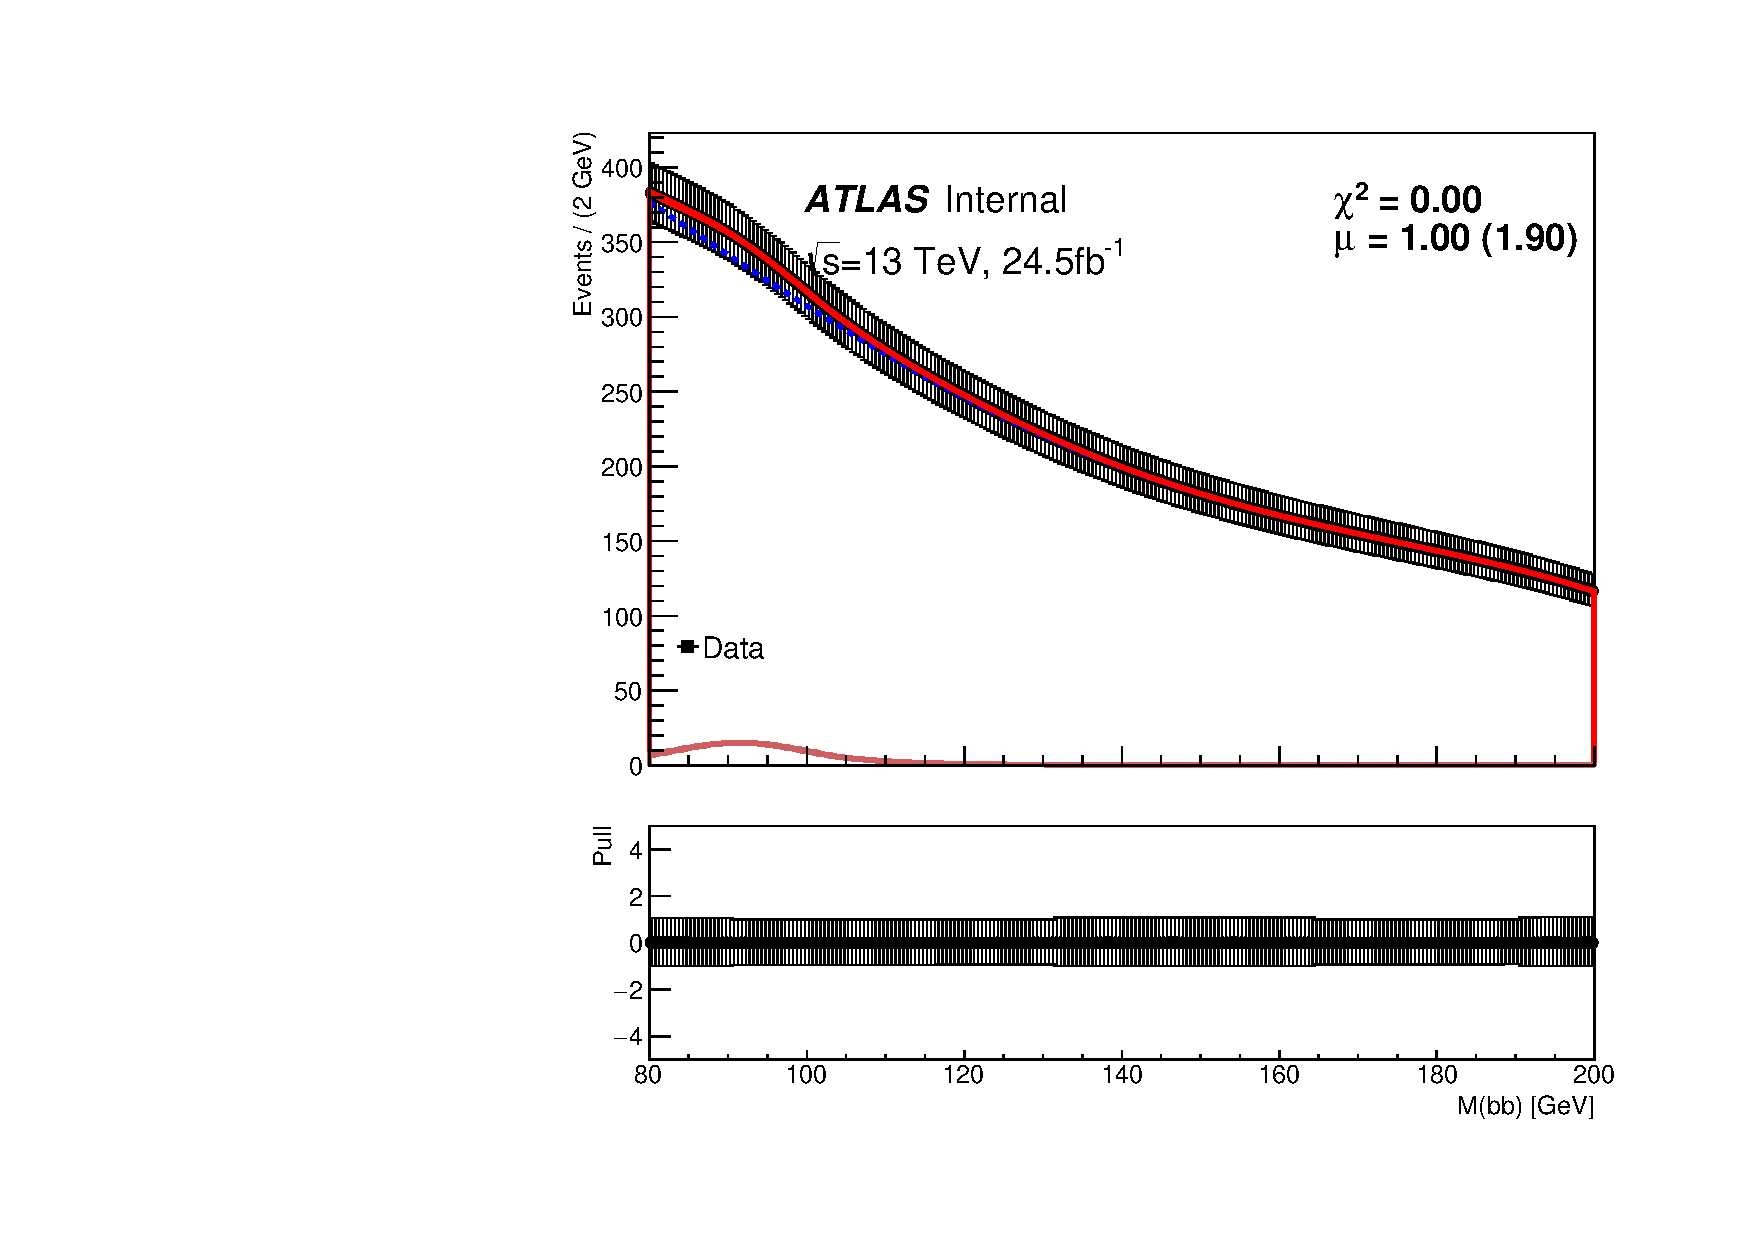
\includegraphics[width=0.48\textwidth]{figures/VBF/Asimov_testVBF_ICHEP_4cen_SRII.pdf}
% 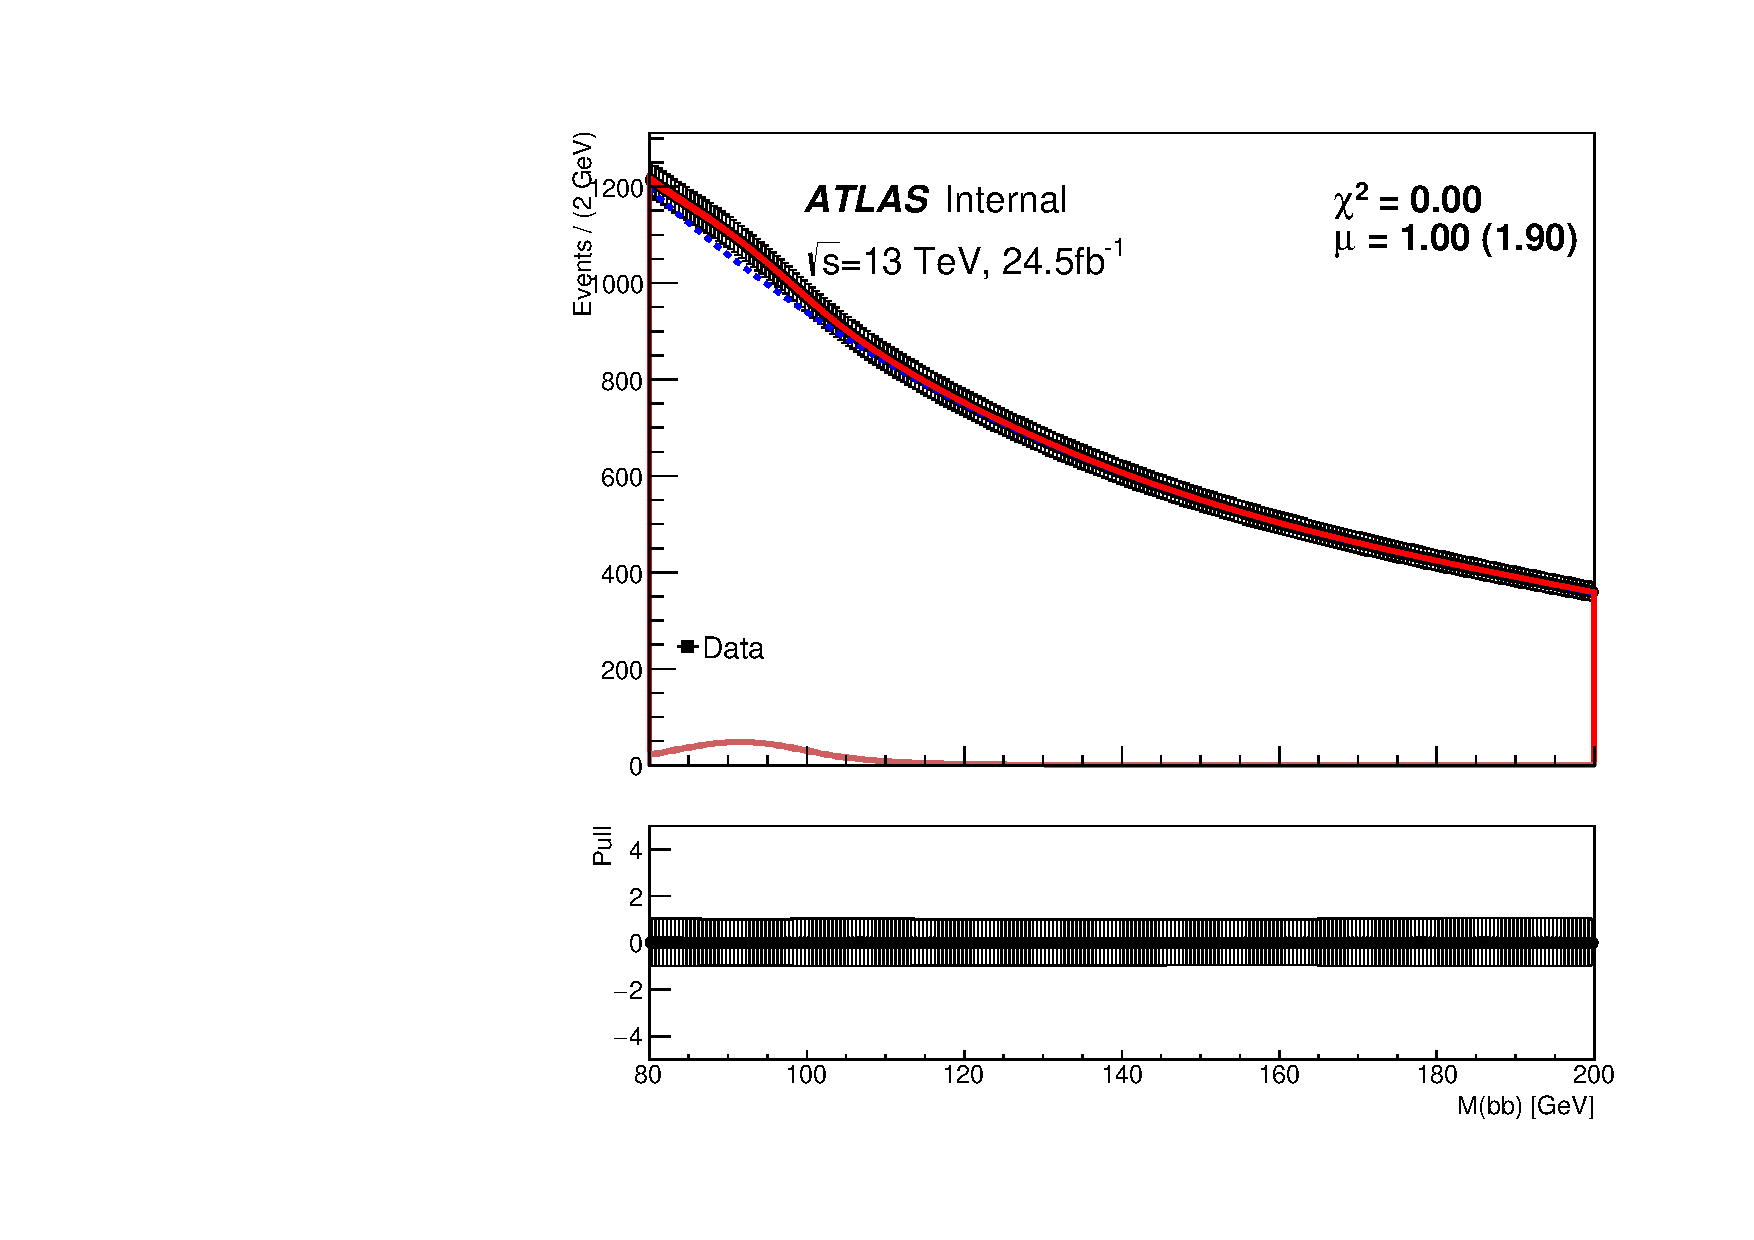
\includegraphics[width=0.48\textwidth]{figures/VBF/Asimov_testVBF_ICHEP_4cen_SRIII.pdf}
% 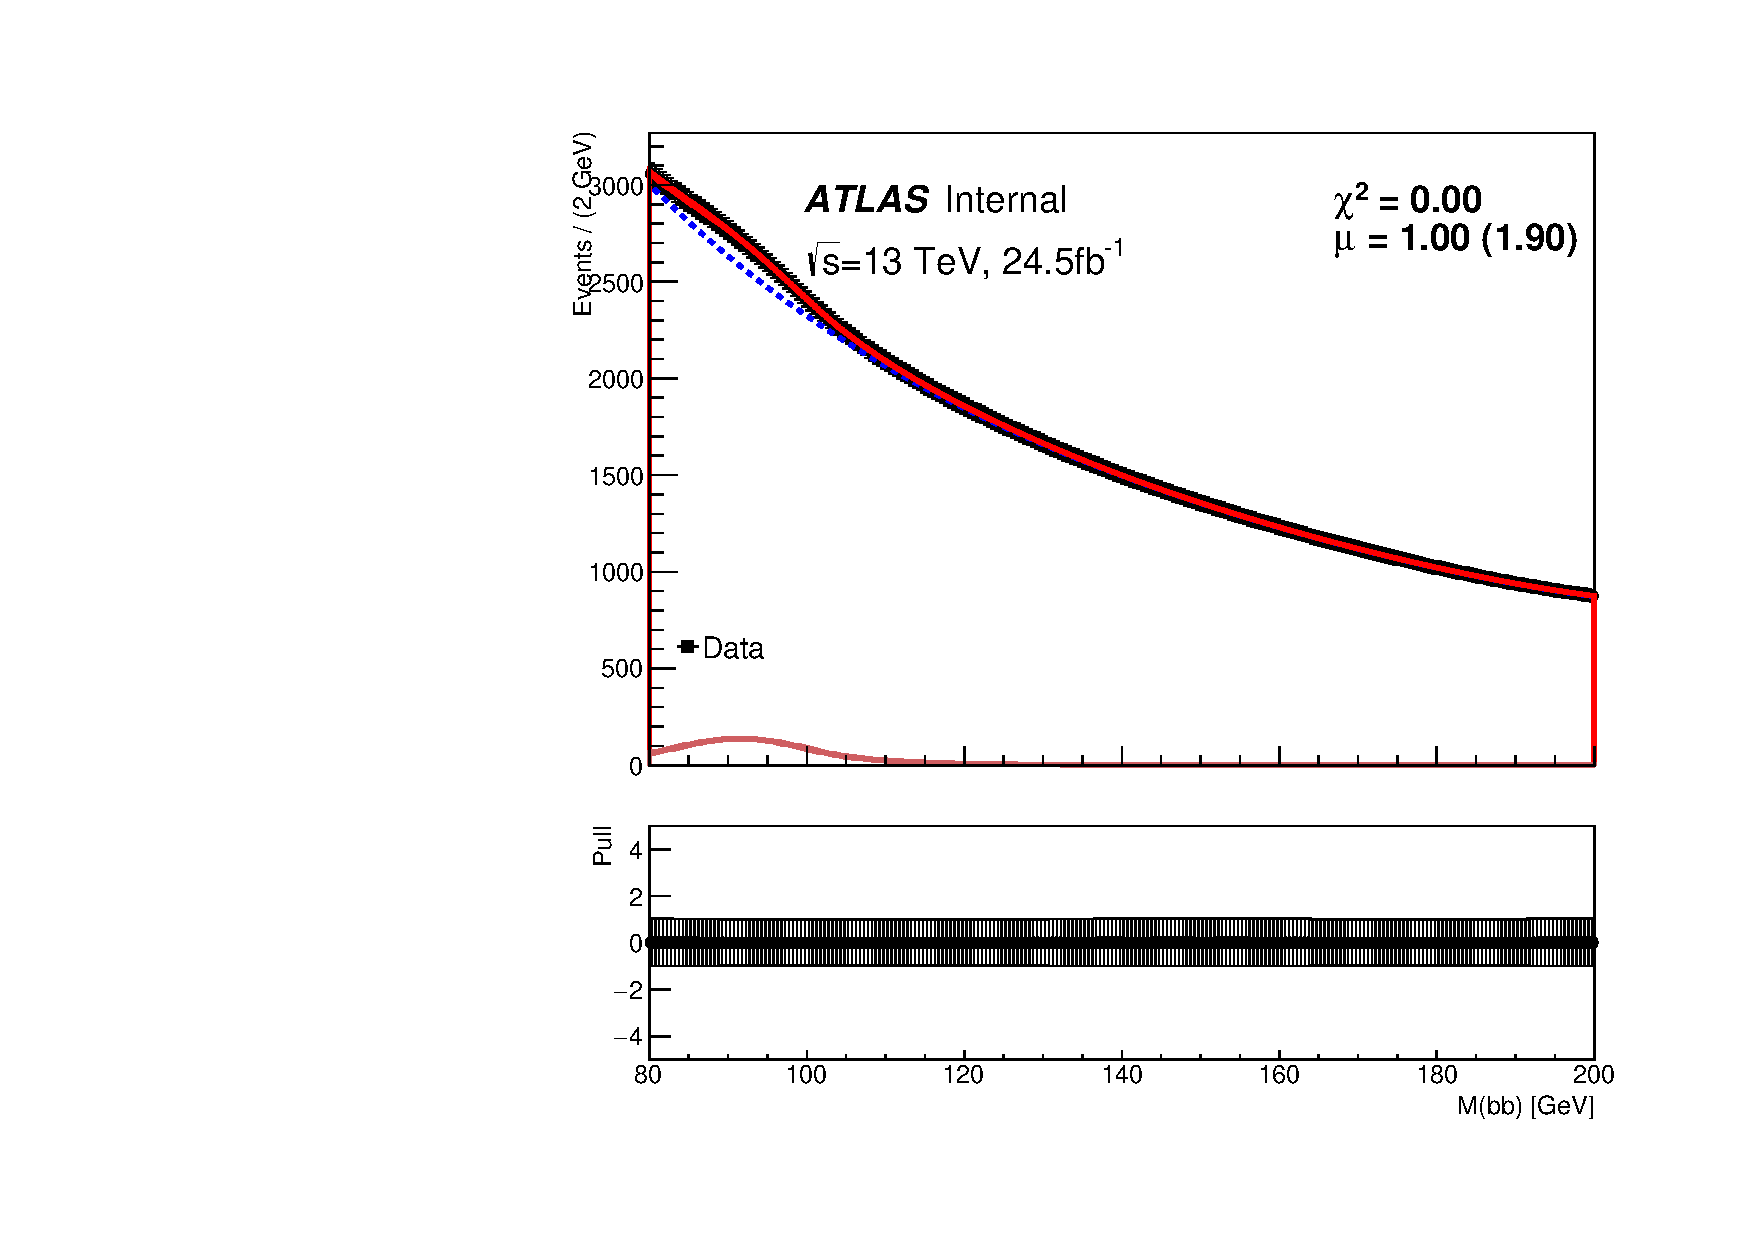
\includegraphics[width=0.48\textwidth]{figures/VBF/Asimov_testVBF_ICHEP_4cen_SRIV.pdf}\\
%
%\caption{Asymptotic Asimov fits for SRI to SRIV for the \fourcentral channel.}
%  \label{fig:4cenAsimov}
%\end{figure}


%\begin{figure}[htbp]
%  \centering
% 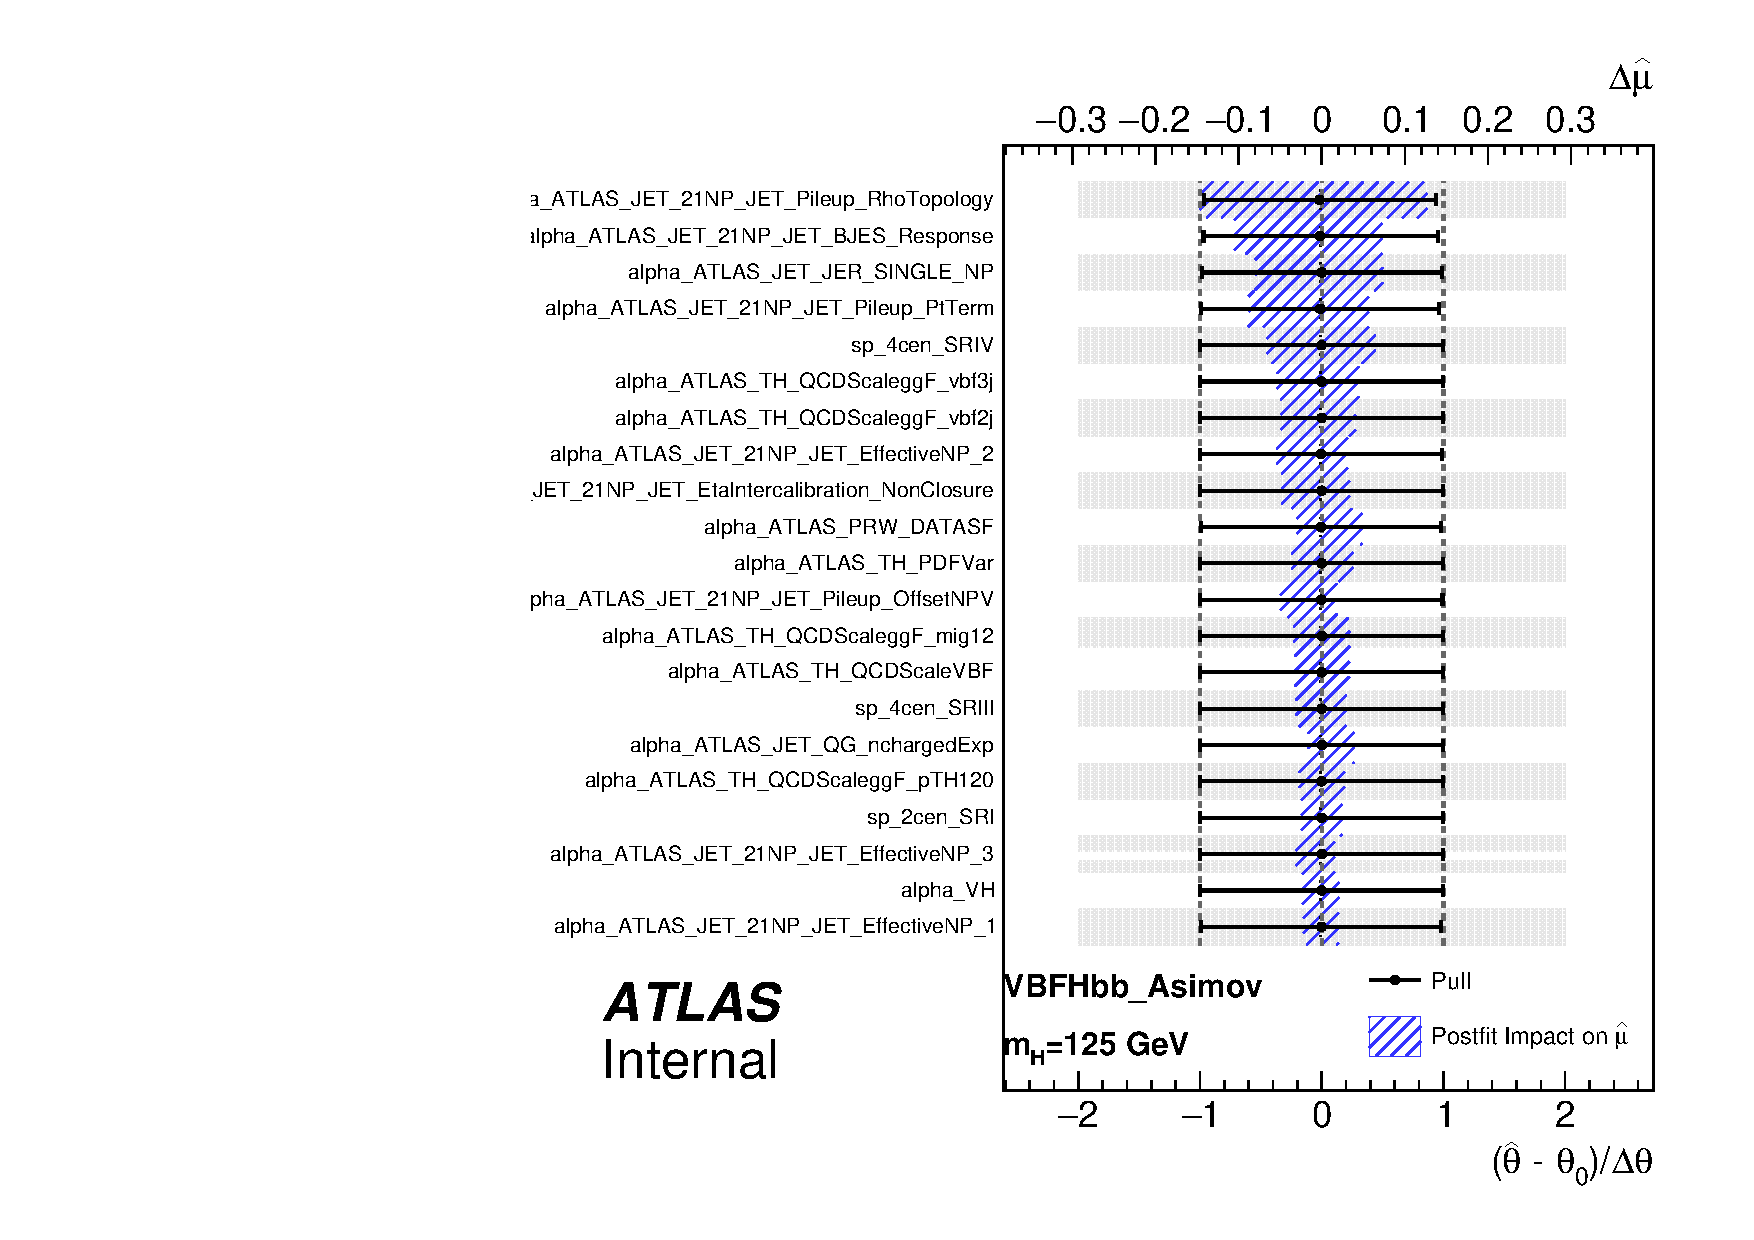
\includegraphics[width=0.9\textwidth]{figures/VBF/VBFHbb_Asimov_pulls_125.pdf}
% \caption{Nuisance parameter post-fit impact ($>1$ \%) and pulls are plotted for the simultaneous Asimov fit. Only the constrained NPs are shown. The uncertainties follow the naming defined in Table. \ref{tab:systnames}. The leading systematics are the jet energy scale and jet energy resolution}
%  \label{fig:pull_asimov}
%\end{figure}


\begin{figure}[htbp]
  \centering
 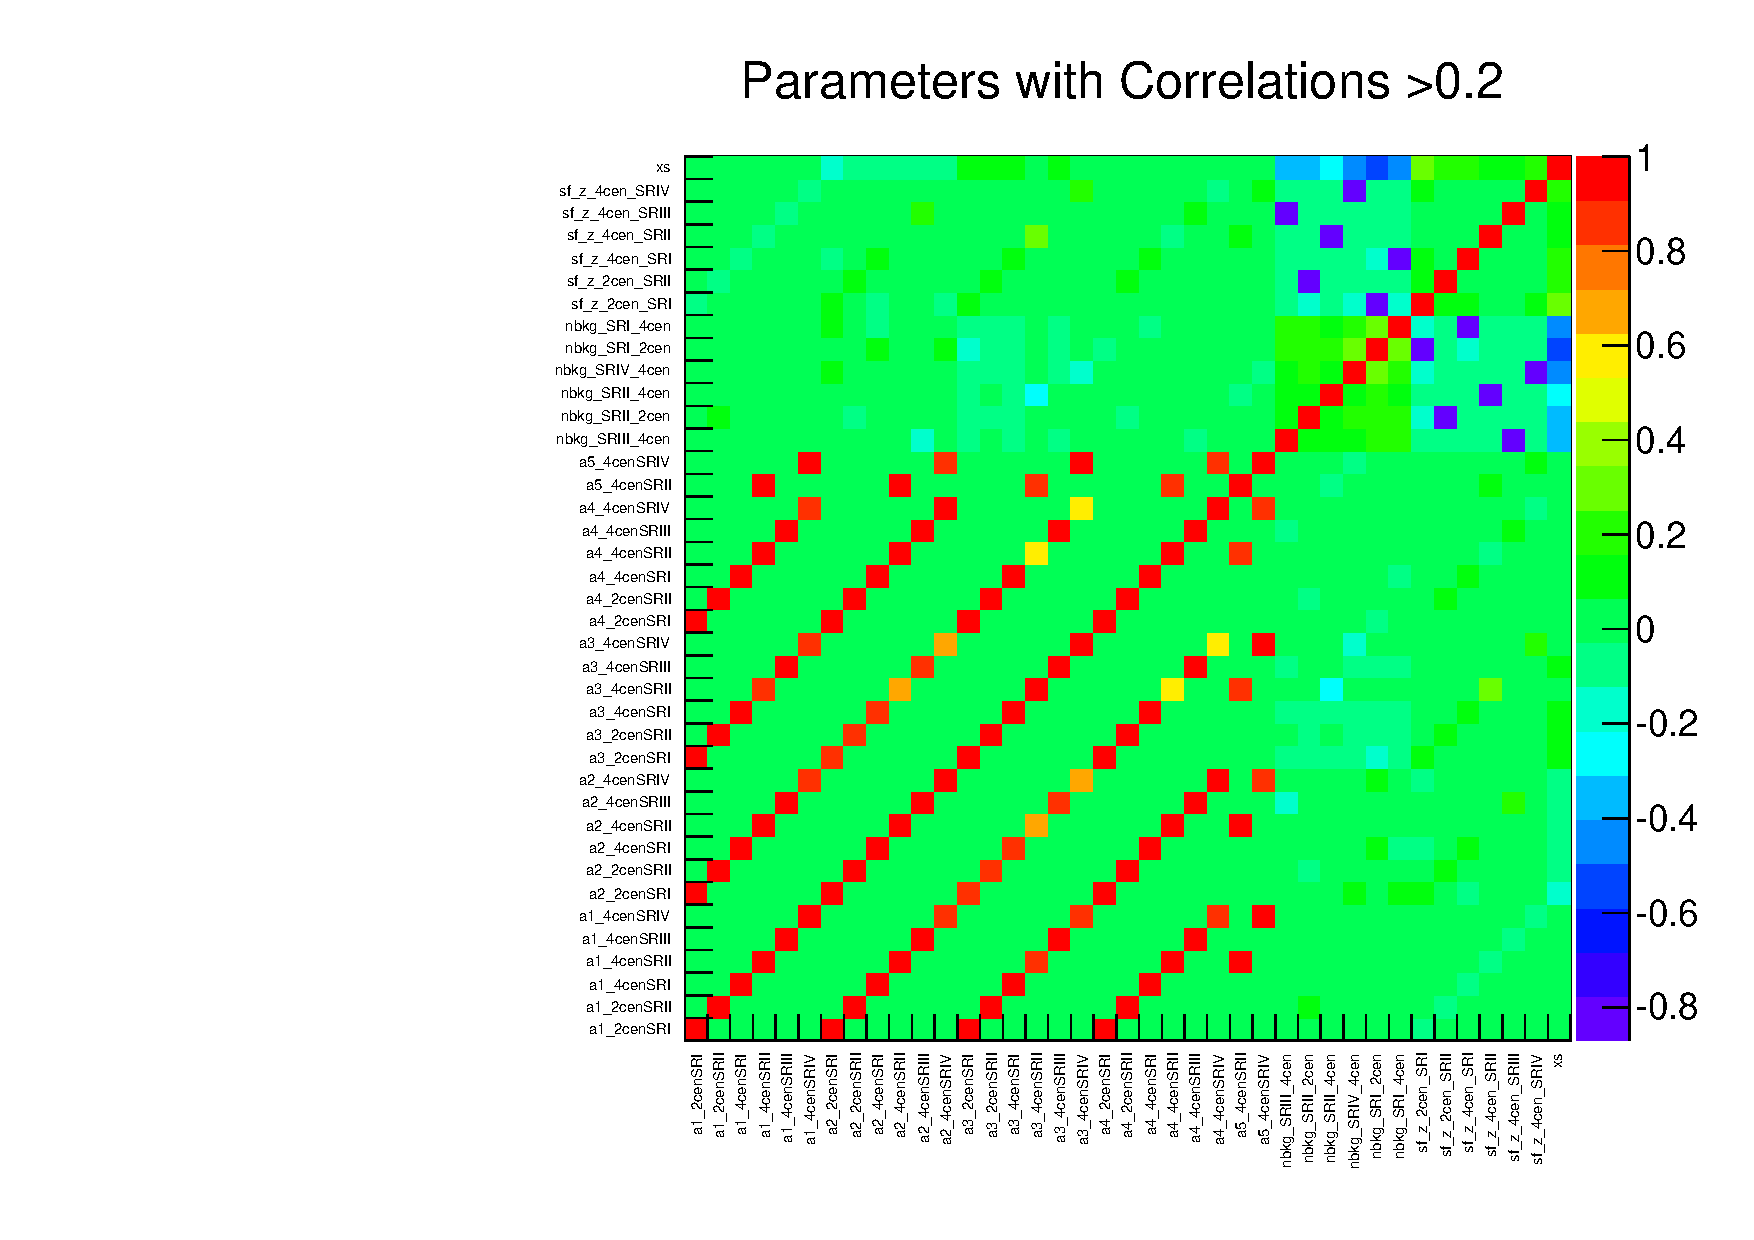
\includegraphics[width=0.8\textwidth]{figures/VBF/Correlation.pdf}

\caption{Nuisance parameter correlation for Asimov fit. Only parameters with $>0.2$ correlations are shown. The background normalizations are pre-fixed as ``nbkg''. The spurious signal size are pre-fixed as ``sp''. The background parameterizations are pre-fixed as ``a1,a2,...,a5'' as defined in \ref{eq:bernstein}. The Z floating parameters are pre-fixed as ``sf\_z''. }
  \label{fig:corr_asimov}
\end{figure}

